My educational journey, profoundly shaped by the dedication and expertise of several remarkable teachers and mentors, have led me to a firm belief in the transformative power of good teaching on a student's life path. Over the years, I have contemplated and reflected on the quintessential pedagogy that balances the act of engaging, conveying, and inspiring. Specifically, in developing my course materials, I am guided by a series of introspective questions that aims at ensuring that the content not only is informative but also stimulates critical thinking.
\begin{quote}
    I continually ask myself five key questions:
    \begin{enumerate}[nosep,leftmargin=*]
        \item What insights will students gather while actively engaging with both my spoken words and the slide content?
        \item What insights will students gather while independently examining the slide content at my lecture pace?
        \item What are the takeaways for students when they revisit the slides on their own time?
        \item How can I guarantee consistency in the key takeaways gathered across these varied learning contexts?
        \item How do I structure the slide content to convey key messages to the students without them directly reading from it?
    \end{enumerate}
\end{quote}
These practices have shaped my teaching philosophy, which emphasizes the effective use of visualization.

\section{Teaching Philosophy}
Visualization is central to my instructional approach, leveraging the human brain's rapid image processing ability, which reportedly surpasses text interpretation by 6x\textendash 600x\footnote{
    Despite the discrepancy with the unfounded internet meme claiming 60,000x, as called out in \emph{The 60,000 Fallacy} (\url{https://policyviz.com/2015/09/17/the-60000-fallacy/}), this is still substantial enough to warrant extra attention to the use of visualization in teaching.
}~\cite{ResearchPictureWorth}.
This capability enables students to extract information from visual aids alongside verbal explanations far more efficiently than text alone, allowing for profound engagement in class. In the realm of STEM education, where abstract theories and complex equations can be overwhelming, visualization serves as a vital bridge, translating intricate ideas into comprehensible and memorable images. It also elegantly addresses the pedagogical challenge of conveying essential concepts without resorting to simply reading from the slides\textemdash a practice that hinders critical thinking. Beyond the immediate classroom benefits, the ability to visualize data and concepts is an indispensable skill for students, one that is increasingly critical in both their academic pursuits and future research careers. Building on this philosophy, I address the challenge of ensuring consistent takeaways from the course materials in different learning contexts\textemdash whether inside or outside the classroom\textemdash by integrating concise bullet points alongside visuals, ensuring key messages being conveyed.

\section{Pitfalls and Lessons Learned}
Designing visuals that effectively encode information demands thoughtful consideration and attention to detail, ensuring accessibility for all learners. Informed by my personal experience with minor color vision deficiency, I am acutely aware of key pitfalls in visual information delivery, such as solely relying on color contrast to embed information. For instance, Fig.~\ref{fig:color} demonstrates how using color as the sole differentiator between two spectra can make the data difficult to interpret for those with color vision impairments. The prevalence of color blindness, affecting approximately 8\% of males and 0.5\% of females~\cite{TypesColourBlindness}, might surprise many. However, this statistic virtually guarantees that in any moderately sized classroom, at least one individual is likely to have a form of color vision deficiency. Acknowledging this, I am committed to employing multiple modes of differentiation in my teaching materials, such as patterns, textures, and annotations, to ensure that all students, regardless of visual ability, have equal access to the information presented.

\begin{figure}[!t]%
    \centering
    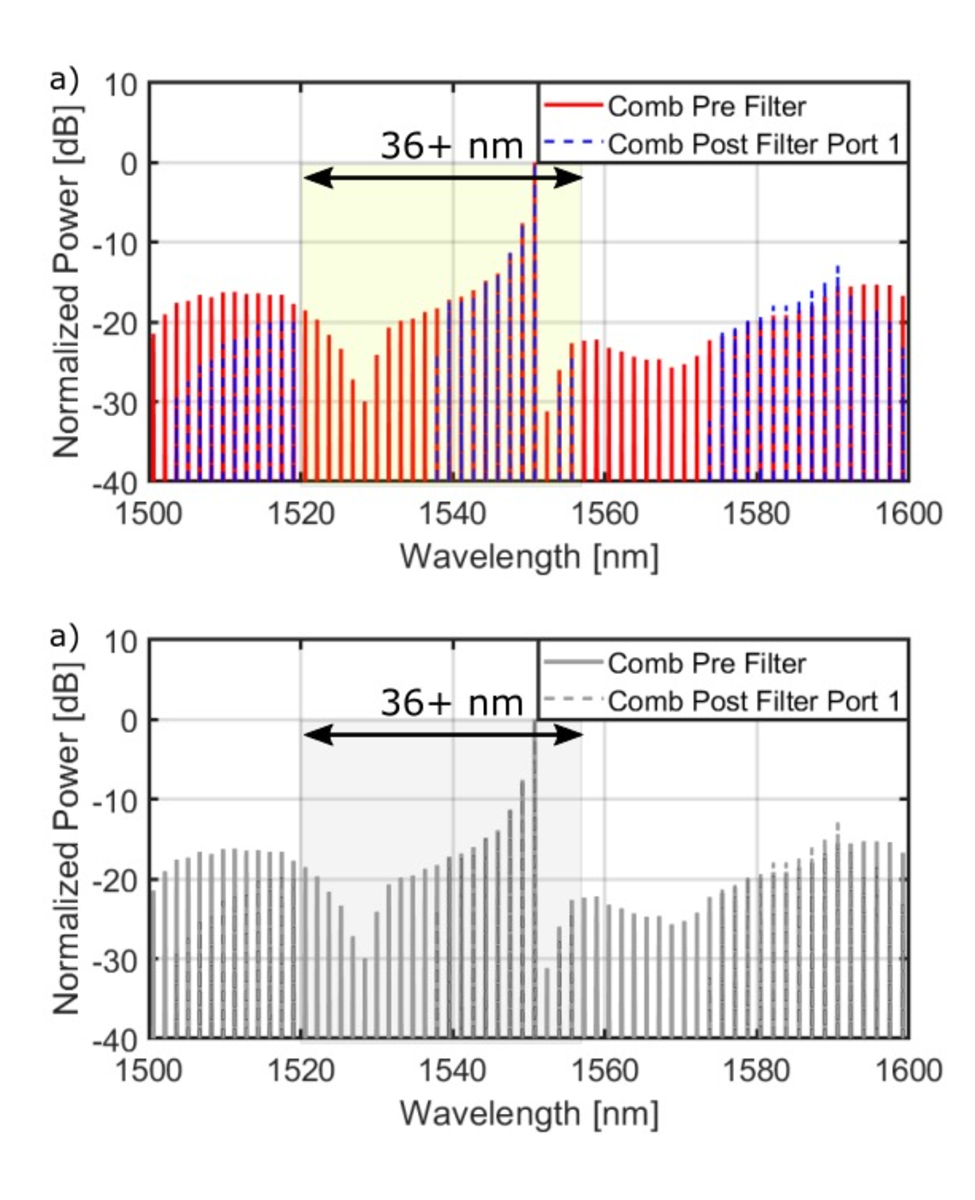
\includegraphics[width=0.95\linewidth]{../../fig/color.pdf}
    \caption{Example of non-robust information encoding solely with color contrast. \textbf{a)}~Two spectra distinguishable by people with normal color vision. \textbf{b)}~Illustrative rendering of the same two spectra possibly perceived by people with color vision deficiency.}
    \label{fig:color}
\end{figure}

\section{Inclusive Teaching}
My commitment to inclusivity extends beyond color vision awareness to embrace all facets of diversity and accessibility in education. I recognize that students come with a broad spectrum of cultural backgrounds, personal histories, and educational experiences, all of which influence their learning needs. In light of this, I will strive to create a classroom environment that is not only physically accessible but also cognitively and culturally welcoming. This entails the use of language that is inclusive and bias-free, as well as the incorporation of diverse examples in my teaching materials, practices that I will regularly reflect on to ensure adherence.


\section{Teaching Plans}
In harmony with the esteemed curriculum of the \appDept{} at the \appSchool{}, I am eager to contribute by teaching a range of courses that intersect with my expertise,%